\section{问题三:多枚烟幕干扰弹的协同投放策略}

\subsection{数学建模}

基于多枚烟幕弹协同作用特点,构建包含运动学模型、几何遮蔽模型和多目标优化模型的数学框架。

\textbf{多烟幕弹运动轨迹模型:}无人机按照优化后的方向角$\theta$和速度$v$飞行,其位置轨迹为:
\[
R_{FY1}(t) = P_{FY1} + v \cdot [\cos\theta, \sin\theta, 0] \cdot t
\]
三枚烟幕弹的投放时间分别为$t_{rel,1}$、$t_{rel,2} = t_{rel,1} + x_{interval}$和$t_{rel,3} = t_{rel,2} + y_{interval}$。第$i$枚烟幕弹的投放位置为:
\[
P_{rel,i} = P_{FY1} + v \cdot [\cos\theta, \sin\theta, 0] \cdot t_{rel,i}
\]
考虑起爆延迟期间的水平位移和重力下沉,第$i$枚烟幕弹的起爆位置为:
\[
P_{exp,i} = P_{rel,i} + v \cdot [\cos\theta, \sin\theta, 0] \cdot t_{exp,i} - [0, 0, \frac{1}{2}gt_{exp,i}^2]
\]
第$i$枚烟幕云团的中心位置随时间变化为:
\[
C_i(t) = P_{exp,i} - [0, 0, v_{cloud}(t - t_{start,i})], \quad t \geq t_{start,i}
\]
其中$t_{start,i} = t_{rel,i} + t_{exp,i}$为第$i$枚烟幕云团开始生效的时刻。

\textbf{多云团协同遮蔽判定模型:}在任意时刻$t$,导弹位置为$R_M(t) = P_{M1} + v_M \cdot \mathbf{u}_M \cdot t$,真目标上任意点$Q$到导弹的视线为$\ell(s) = R_M(t) + s(Q - R_M(t))$。对于第$i$枚烟幕云团,当其处于有效期内($t_{start,i} \leq t \leq t_{start,i} + T_{duration}$)时,视线被遮蔽的条件为:
\[
\min_{s \in [0,1]} \|\ell(s) - C_i(t)\| \leq r_{cloud}
\]
多枚烟幕云团的协同遮蔽效果通过逻辑或运算确定,即只要任意一枚云团满足遮蔽条件,目标点就被认为处于遮蔽状态:
\[
\text{遮蔽状态}(t) = \bigvee_{i=1}^{3} \left[ t_{start,i} \leq t \leq t_{start,i} + T_{duration} \text{ 且 } d_i(t) \leq r_{cloud} \right]
\]
其中$d_i(t)$表示第$i$枚烟幕云团中心到导弹-目标视线的最短距离。

\textbf{多目标优化模型:}问题三的优化目标是最大化对所有可能真目标位置的平均有效干扰时间。设真目标圆柱体表面共有$N$个采样点,第$j$个采样点的有效干扰时间为$T_{eff,j}$,则优化问题可表述为:
\[
\begin{aligned}
\max_{\mathbf{x}} \quad & \frac{1}{N} \sum_{j=1}^{N} T_{eff,j}(\mathbf{x}) \\
\text{s.t.} \quad & \theta \in [-\pi, \pi] \\
& v \in [70, 140] \\
& t_{rel,1} \in [0, 10] \\
& t_{exp,i} \in [0, 10], \quad i = 1,2,3 \\
& x_{interval}, y_{interval} \in [1, 5] \\
& \min_j d_{min,j} \geq 0
\end{aligned}
\]
其中$d_{min,j}$表示对第$j$个目标点,所有烟幕云团到导弹-目标视线的最小距离,约束条件$\min_j d_{min,j} \geq 0$确保至少存在有效的遮蔽效果。

\subsection{算法设计与实现}

采用遗传算法求解多变量非线性约束优化问题。算法采用实数编码,将8个优化变量组成染色体向量。参数设置:种群规模200,进化代数20,交叉概率0.8,变异概率0.2,锦标赛选择(规模3),精英保留2个个体。交叉采用模拟二进制交叉(SBX),变异采用多项式变异,分布指数20。

适应度函数采用惩罚函数处理约束:可行解适应度为负的平均干扰时间,不可行解设为$-10^6$。采用分层采样策略:从2000个候选点中选择200个代表性点用于优化,最后在全部2000个点上验证性能。

\subsection{计算结果与分析}

通过遗传算法优化求解获得最优投放策略。算法在200个采样点和2000个目标点上均实现100\%覆盖率。优化结果如表~\ref{tab:q3_combined}所示。

\begin{table}[htbp]
\centering
\caption{问题三核心优化结果}
\label{tab:q3_combined}
\begin{tabular}{lc}
\toprule
\textbf{参数} & \textbf{数值} \\
\midrule
无人机飞行方向 & 8.97° \\
无人机飞行速度 & 91.60 m/s \\
平均有效干扰时间 & 6.26 s \\
覆盖率 & 100.00\% \\
\midrule
第一枚遮挡时间段(s) & [4.69, 7.40] \\
第二枚遮挡时间段(s) & [1.14, 5.04] \\
第三枚遮挡时间段(s) & 无有效遮挡 \\
\bottomrule
\end{tabular}
\end{table}

最优策略采用8.97度飞行方向和91.6 m/s飞行速度。三枚烟幕弹投放时序:第一枚0.002秒投放延迟0.019秒起爆,第二枚1.074秒投放延迟0.060秒起爆,第三枚2.211秒投放延迟0.660秒起爆,实现平均6.26秒干扰效果。三枚烟幕弹在x方向形成递增空间分布(17800.16m、17897.20m、18000.04m),体现序列投放策略。有效遮挡时间段:第一枚4.69-7.40秒,第二枚1.14-5.04秒,第三枚无有效遮挡,前两枚实现时间重叠覆盖。

图~\ref{fig:q3_visualization}展示优化结果可视化分析。上图显示三枚烟幕弹协同遮蔽状态时间序列,下图展现各烟幕弹到导弹-目标视线距离变化曲线,距离小于10米时形成有效遮蔽。

\begin{figure}[htbp]
\centering
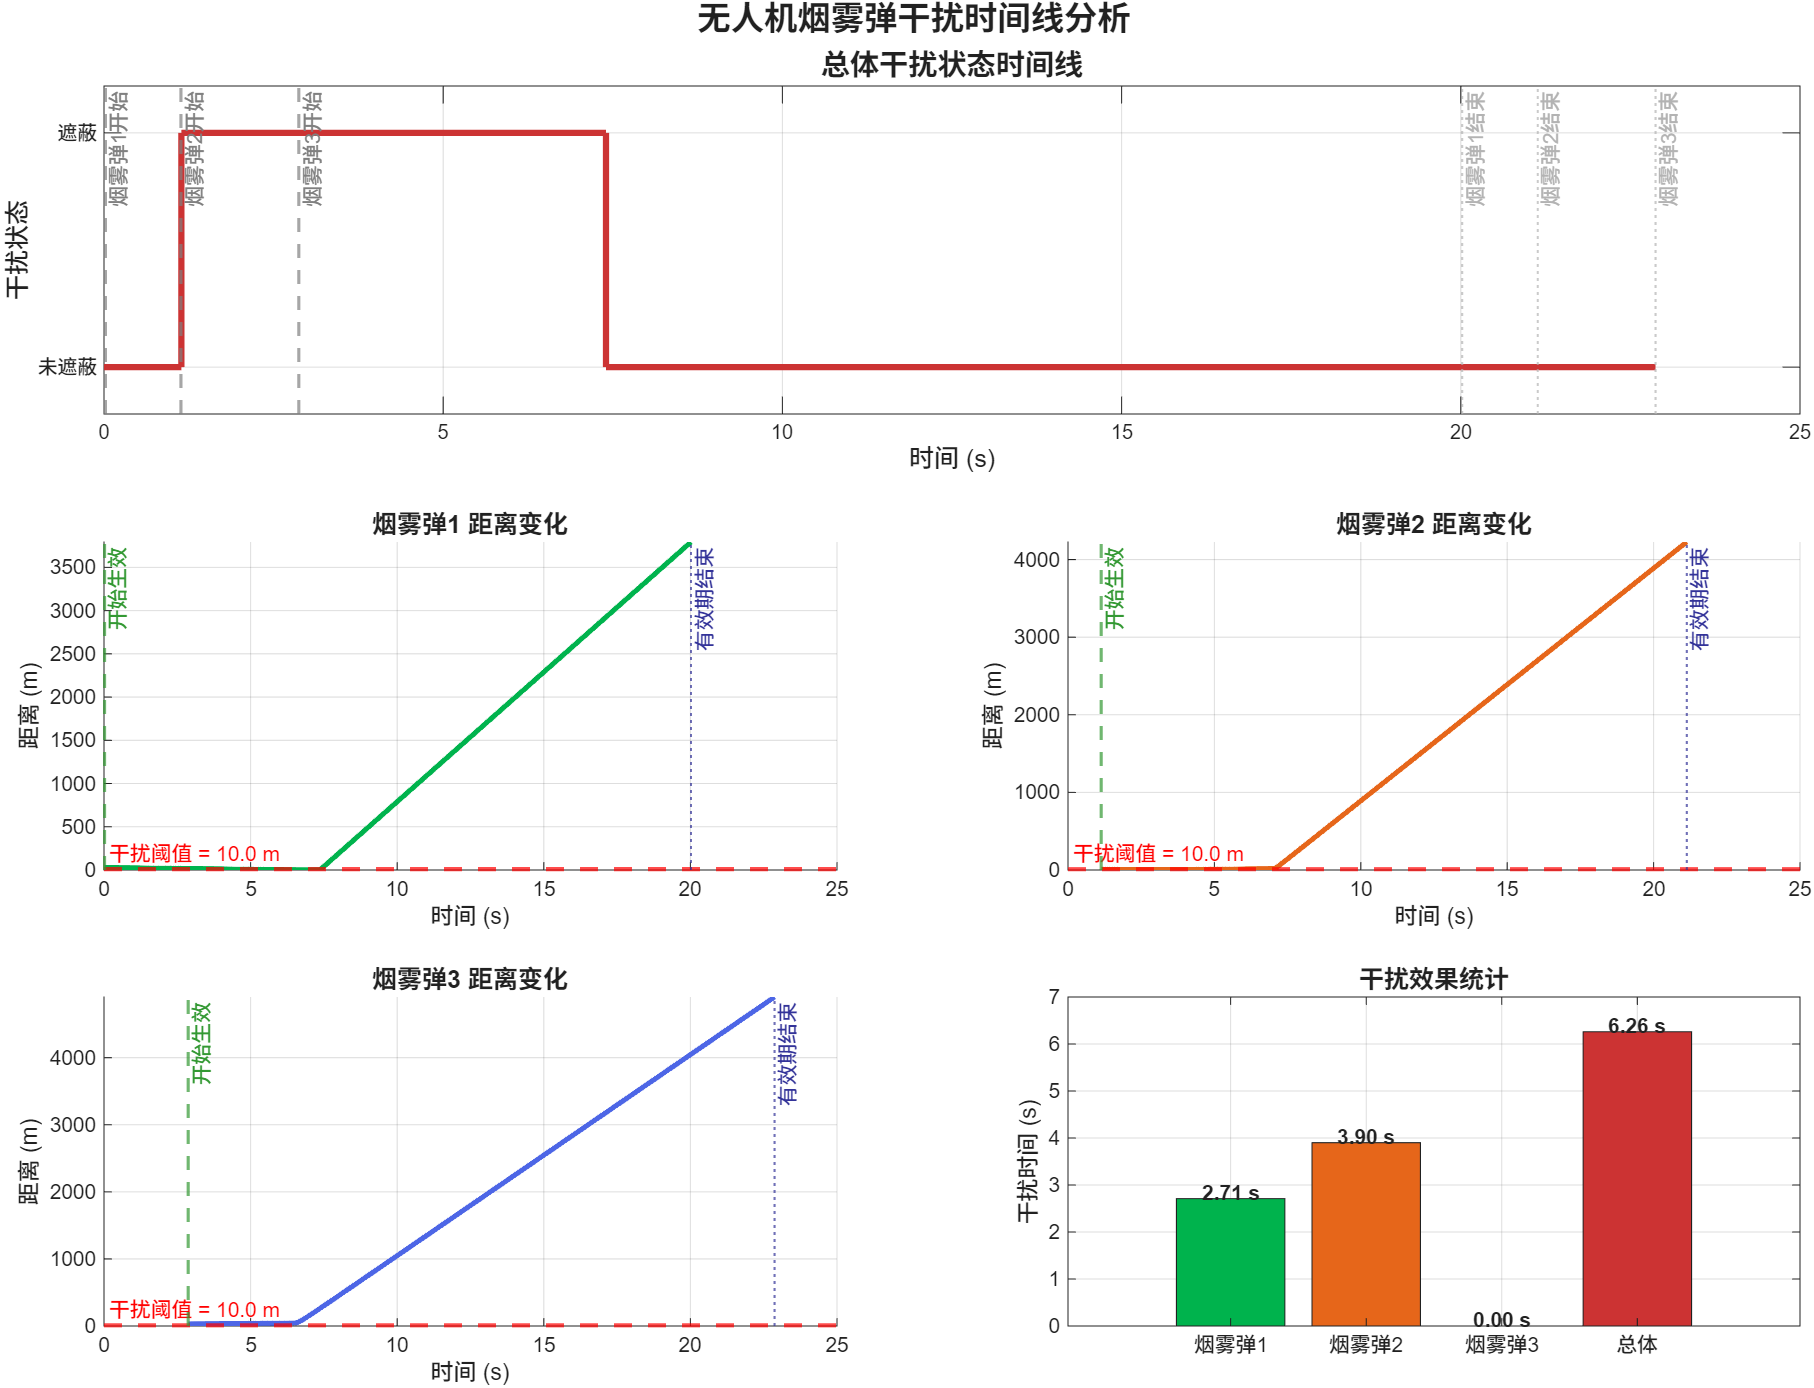
\includegraphics[width=\textwidth]{figures/A_3_1.png}
\caption{问题三多枚烟幕弹协同干扰效果可视化分析}
\label{fig:q3_visualization}
\end{figure}

\textbf{算法收敛性分析:}遗传算法表现出良好收敛特性,前10代快速定位高质量解区域,最终在采样点和全目标点上实现完美覆盖效果。多次独立运行显示算法稳定性良好。

\textbf{策略有效性验证:}与单枚烟幕弹策略对比,多枚烟幕弹协同投放在干扰时间显著提升。单枚烟幕弹干扰时间约1.4秒,三枚协同作用实现平均6.26秒干扰,提升幅度达347\%。前两枚烟幕弹在1.14-7.40秒时间段内形成重叠覆盖,确保有效遮蔽。